\documentclass[a4paper, 12pt]{article}
\usepackage{titling}
\usepackage{array}
\usepackage{booktabs}
\usepackage{enumitem}
\usepackage{graphicx}
\usepackage{hyperref}
\usepackage{amssymb}
%\usepackage{mathtools}
\usepackage{listings}
\usepackage{amsmath}
\usepackage{color} %red, green, blue, yellow, cyan, magenta, black, white
\setlength{\heavyrulewidth}{1.5pt}
\setlength{\abovetopsep}{4pt}
\setlength{\parindent}{0pt}
\graphicspath{{.}}
\usepackage{float}
\usepackage[margin=1in]{geometry}
\definecolor{mygreen}{RGB}{28,172,0} % color values Red, Green, Blue
\definecolor{mylilas}{RGB}{170,55,241}
% Must be after geometry
\usepackage{fancyhdr}
\pagestyle{fancy}
\fancyhf{}
\rhead{NN Homework 5}
\lhead{P.Lukin, E. Ovchinnikova}
\cfoot{\thepage}

\setlength{\droptitle}{-5em}

\title{Neural Networks  \\
				- Homework 5 -}
\author{Petr Lukin, Evgeniya Ovchinnikova}
\date{Lecture date: 31 October 2016}

\begin{document}

%-------------------------------------------------------------------------------
\lstset{language=Matlab,%
    %basicstyle=\color{red},
    breaklines=true,%
    morekeywords={matlab2tikz},
    keywordstyle=\color{blue},%
    morekeywords=[2]{1}, keywordstyle=[2]{\color{black}},
    identifierstyle=\color{black},%
    stringstyle=\color{mylilas},
    commentstyle=\color{mygreen},%
    showstringspaces=false,%without this there will be a symbol in the places where there is a space
    numbers=left,%
    numberstyle={\tiny \color{black}},% size of the numbers
    numbersep=9pt, % this defines how far the numbers are from the text
    emph=[1]{break},emphstyle=[1]\color{red}, %some words to emphasise
    %emph=[2]{word1,word2}, emphstyle=[2]{style},
}

%-------------------------------------------------------------------------------

\maketitle

\section{Mind map}

\begin{figure}[h]
  \centering
  \caption{Mind map. Chapter 4 (first part) from Haykin’s book. A zoomed version is attached as MultilayerPerceptron.png \label{fig:MultilayerPerceptron}}
  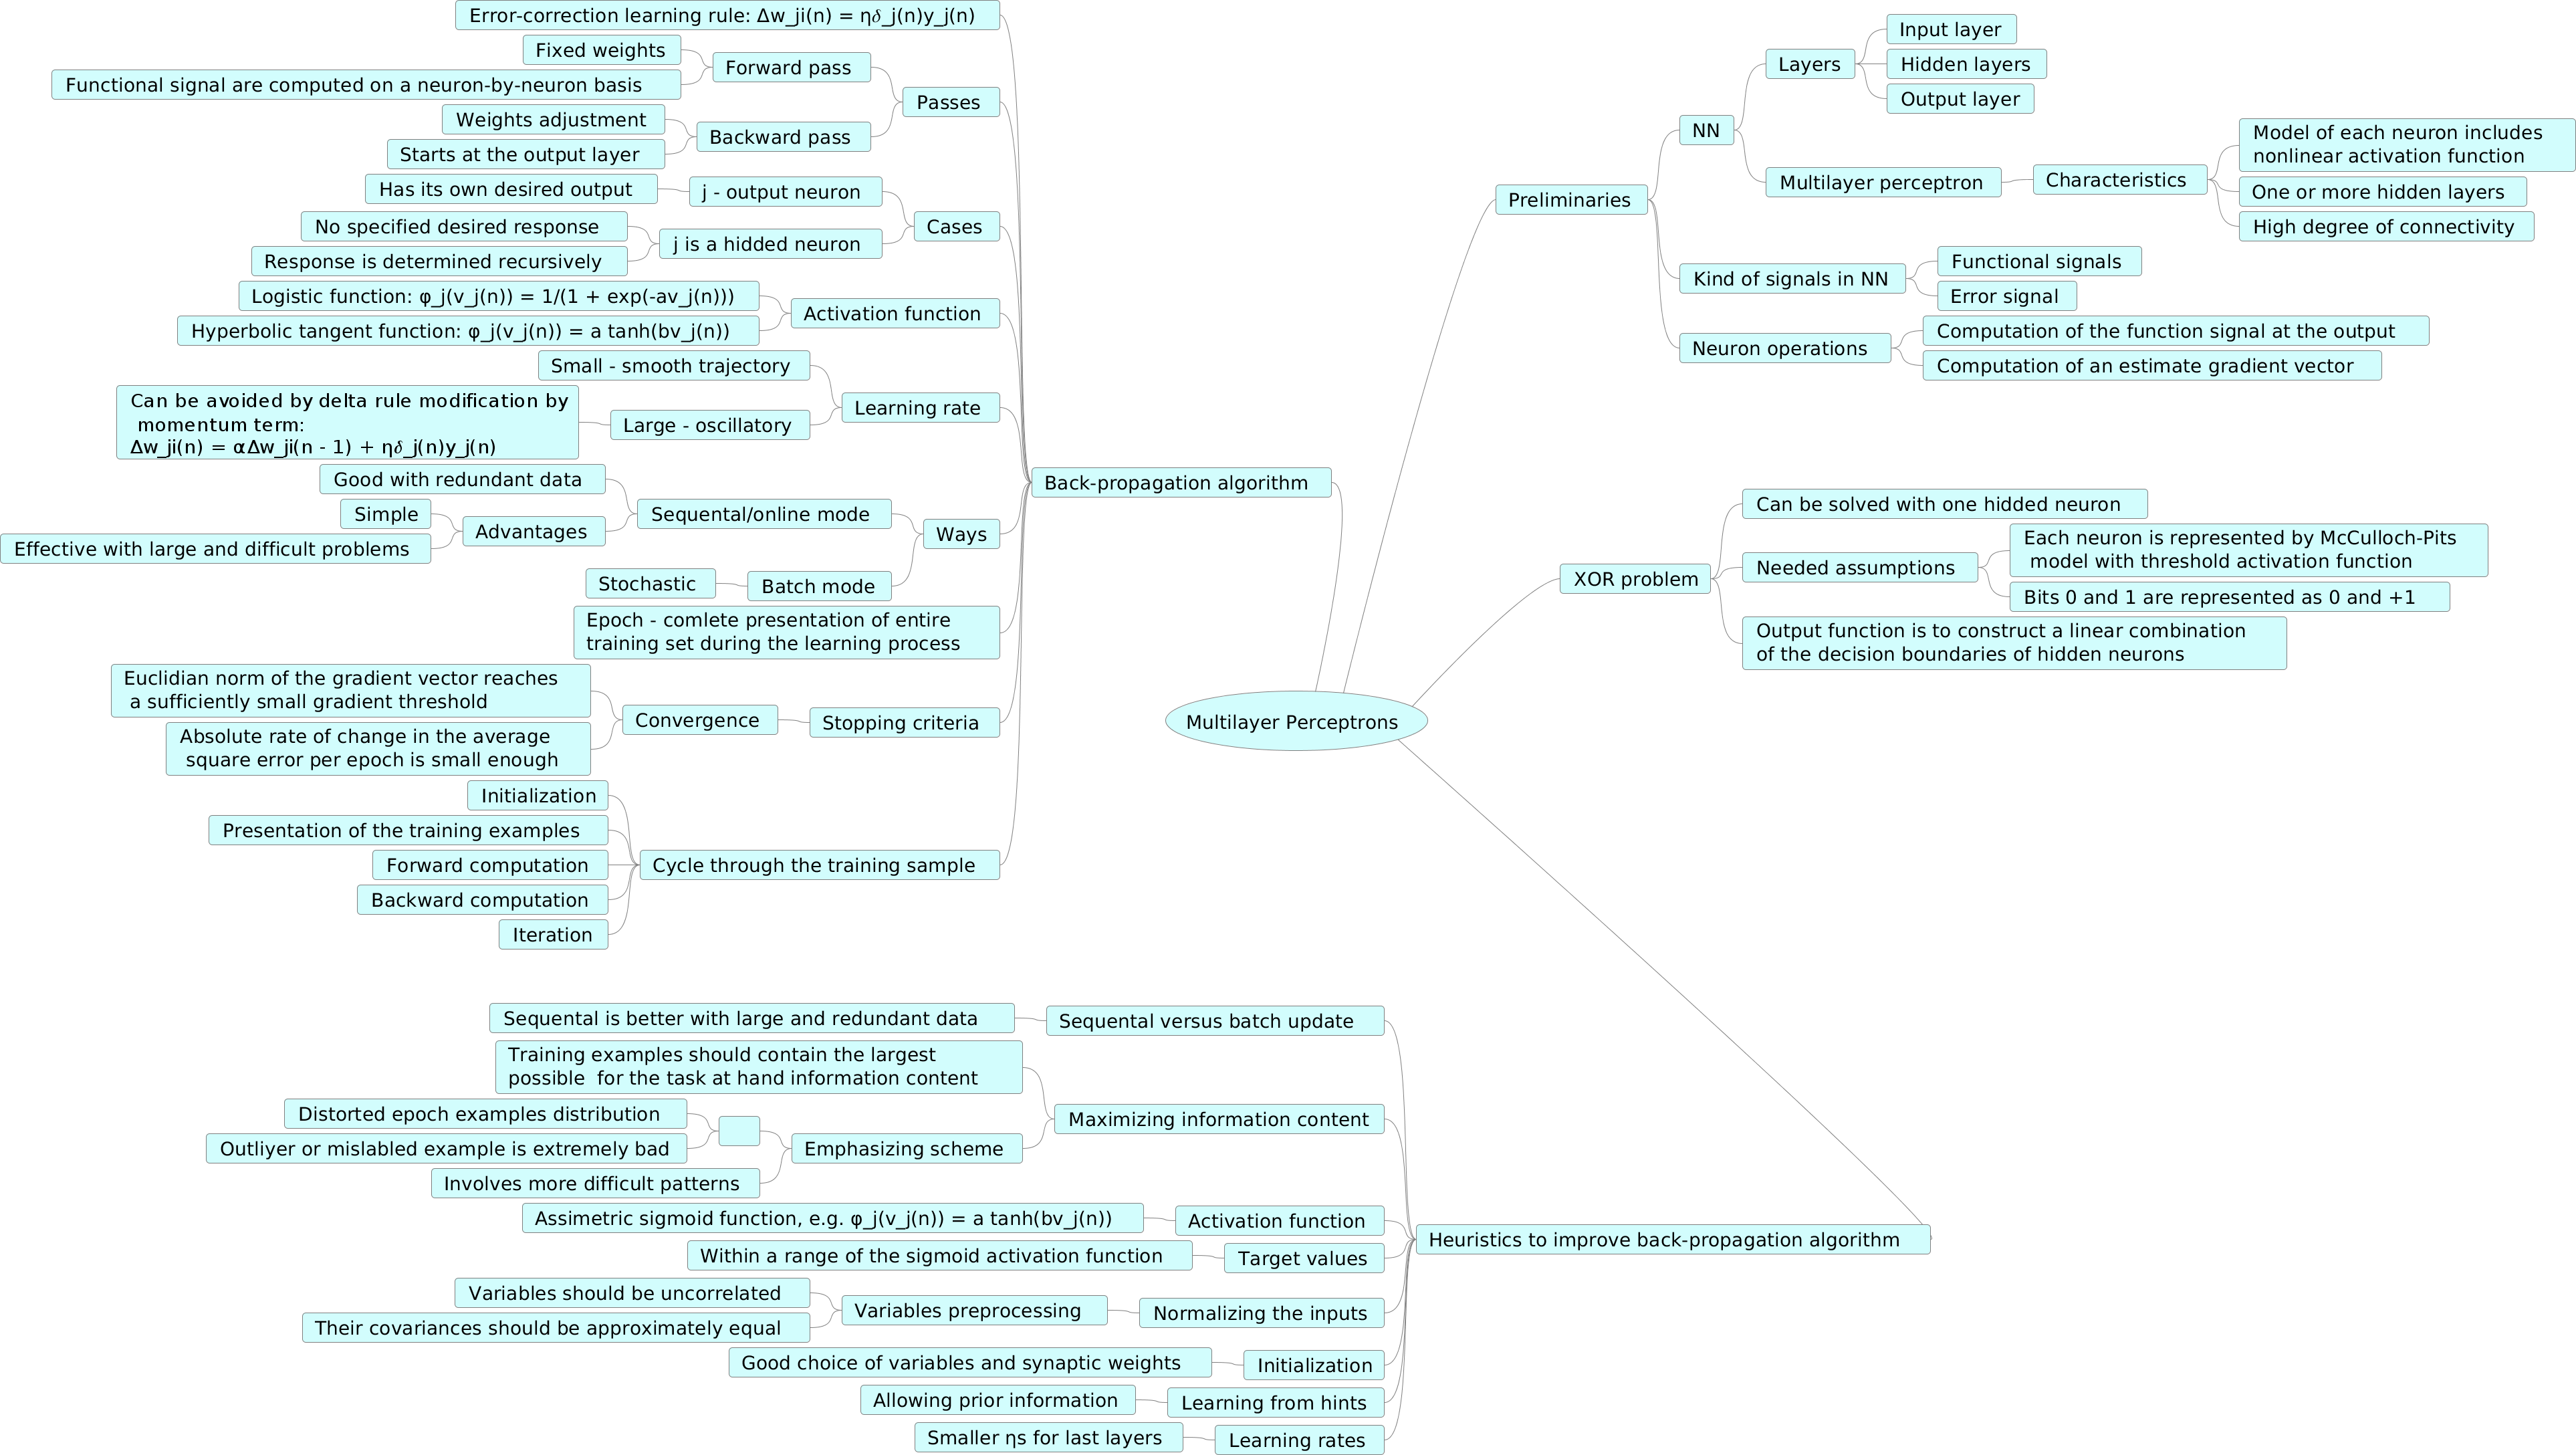
\includegraphics[width=1.1\textwidth]{MultilayerPerceptron}
\end{figure}

\section{Exercises}

\subsection{Exercise 2}

For this task you have to program the back-propogation (BP) for multi layered perceptron (MLP). Design your implementation for general NN with arbitrary many hidden layers. The test case is as follows:  2-2-1 multi layered perceptron depicted in Fig. \ref{fig:perceptron} (MLP) with sigmoid activation function on XOR data that is shown in Fig.\ref{fig:perceptronLinearAnalysis}. \\

\begin{figure}[h]
  \centering
  \caption{2-2-1 multi layered perceptron \label{fig:perceptron}}
  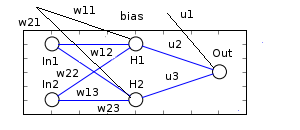
\includegraphics[width=0.4\textwidth]{perceptron}
\end{figure}

\begin{figure}[h]
  \centering
  \caption{XOR values, blue - 0, red - 1 \label{fig:perceptronLinearAnalysis}}
  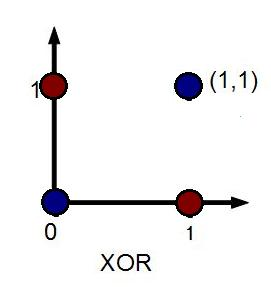
\includegraphics[width=0.2\textwidth]{perceptronLinearAnalysis}
\end{figure}

a. Experiments with initial weights\\

i. Train the network with zero initial weights i.e. $w_{ij}$ = 0.\\

ii. Train with random initial weights\\

Compare and comment on the convergence.\\

b. Experiment with different learning rates e.g. 0.1, 0.3, 0.5, 0.9.\\

Compare the convergence and plot some resulting surfaces. You are not allowed to use any neural network toolbox for this solution.\\

NB: If you fail to implement the general case in order to get the full points it is sufficient to implement only the use case (2-2-1 MLP)\\

Solution:\\

We've used the following rule for weights update:\\

$\Delta w_{ij}(n) = \alpha  \Delta w_{ij}(n-1) + (1-\alpha)\eta \delta_j o_i$,\\
where i, j are indices of neurons corresponding to the weights, $\delta$s are errors, o - output of the neuron, $\eta$ - learning rate and $\alpha$ -  a small constant.\\
$w_{ij}(n) = w_{ij}(n - 1) + \Delta w_{ij}(n)$ \\

It is important to mention that we've added a bias, because without it the results of learning we not satisfying.\\

We've used the following Python code:

\lstset{language=Python}
\begin{lstlisting}[frame=single]

import numpy as np
import matplotlib.pyplot as plt
%matplotlib inline

#XOR input and output, constants
bias = -1
x = np.array([[0.0,0.0,bias],[0.0,1.0,bias],[1.0,0.0,bias],[1.0,1.0,bias]])
y = np.array([0.0,1.0,1.0,0.0])
eta1 = 0.1
eta2 = 0.3
eta3 = 0.5
eta4 = 0.9
alpha = 0.05

number_of_steps = 10000

#sigmoid function
def f(x):
    return 1/(1 + np.exp(-x))
    
def perceptron(w1, w2, u, eta):
    dw1 = np.array([0,0,0])
    dw2 = np.array([0,0,0])
    du = np.array([0,0,0])
    err = 111
    iter = 0

    while(abs(err)>0.02): # for zero weights - "for steps in range(number_of_steps)"
        out = [] 
        iter += 1
        for i in range(len(y)):
            o_in1 = f(np.dot(x[i], w1))
            o_in2 = f(np.dot(x[i], w2))
            intermediate_out = np.array([o_in1, o_in2, bias])
            o_out = f(np.dot(intermediate_out, u))
  
            delta_out = o_out * (y[i] - o_out) *  (1 -o_out)
            err = y[i] - o_out
            delta_h1 = o_in1 * (1 - o_in1) * u[0] * delta_out
            delta_h2 = o_in2 * (1 - o_in2) * u[1] * delta_out
            for j in range(3):
                u[j] = alpha*du[j] + u[j] + (1 - alpha)*eta * delta_out * intermediate_out[j]
                w1[j] = alpha*dw1[j] + w1[j] + (1 - alpha)*eta * delta_h1 * x[i][j]
                w2[j] = alpha*dw2[j] + w2[j] + (1 - alpha)*eta * delta_h2 * x[i][j] 
                du[j] = alpha*du[j] + (1 - alpha)*eta * delta_out * intermediate_out[j]
                dw1[j] = alpha*dw1[j] + (1 - alpha)*eta * delta_h1 * x[i][j] 
                dw2[j] = alpha*dw2[j] + (1 - alpha)*eta * delta_h2 * x[i][j] 
            out.append(o_out) 
    output = ["%.3f" % element for element in out]
    print "iterations"
    print iter
    return output

# random initial weights, 3 - because of the bias

w1_rnd = np.array([np.random.random() for i in range(3)])
w2_rnd = np.array([np.random.random() for i in range(3)])
u_rnd = np.array([np.random.random() for i in range(3)])

print "eta1"
print perceptron(w1_rnd, w2_rnd, u_rnd, eta1)
print "eta2"
print perceptron(w1_rnd, w2_rnd, u_rnd, eta2)
print "eta3"
print perceptron(w1_rnd, w2_rnd, u_rnd, eta3)
print "eta4"
print perceptron(w1_rnd, w2_rnd, u_rnd, eta4)

# zero initial weights
w1_zero = np.array([0,0,0])
w2_zero = np.array([0,0,0])
u_zero = np.array([0,0,0])

print "eta1"
print perceptron(w1_zero, w2_zero, u_zero, eta1)
print "eta2"
print perceptron(w1_zero, w2_zero, u_zero, eta2)
print "eta3"
print perceptron(w1_zero, w2_zero, u_zero, eta3)
print "eta4"
print perceptron(w1_zero, w2_zero, u_zero, eta4)
\end{lstlisting}

The expected outputs for the following inputs [[0,0][0,1][1,0][1,1]] are [0, 1 ,1 ,0].

For zero initial weights we've obtained the following (with a fixed and large number of steps):

\lstset{language=Python}
\begin{lstlisting}[frame=single]
eta1
['0.500', '0.500', '0.500', '0.500']
eta2
['0.500', '0.500', '0.500', '0.500']
eta3
['0.500', '0.500', '0.500', '0.500']
eta4
['0.500', '0.500', '0.500', '0.500']
\end{lstlisting}

So, we can conclude that the network cannot be taught using zero initial weights. So, it can't converge.\\

For random weights we used $\eta$s 0.1 (eta1), 0.3 (eta2), 0.5 (eta3), 0.9 (eta4) and 1.5. We obtained the following:
\lstset{language=Python}
\begin{lstlisting}[frame=single]
eta1
iterations
39710
['0.022', '0.981', '0.981', '0.020']
eta2
iterations
9
['0.022', '0.981', '0.981', '0.020']
eta3
iterations
6
['0.022', '0.981', '0.981', '0.020']
eta4
iterations
6
['0.022', '0.981', '0.981', '0.020']
eta4 = 1
iterations
7
['0.022', '0.981', '0.981', '0.020']
\end{lstlisting}

We can see that with increase of $\eta$ the learning is better and converges faster till certain value of $\eta$ (around 0.8-0.9 here), but after it learns more slow.\\

We have created a net of points from (0,0) to (1,1) and applied the perceptron to these points. For that we've modified the code in the following way:

\lstset{language=Python}
\begin{lstlisting}[frame=single]
def classify(x,w1,w2,u):
    x = np.append(x,-1)
    o_in1 = f(np.dot(x, w1))
    o_in2 = f(np.dot(x, w2))
    intermediate_out = np.array([o_in1, o_in2, -1])
    o_out = f(np.dot(intermediate_out, u))
    return o_out
    
from matplotlib import pyplot
from math import cos, sin, atan

%matplotlib inline

points_to_classify = np.zeros([11,11,2])

for i in range(11):
    for j in range(11):
        points_to_classify[i][j][0] = i / 10.0
        points_to_classify[i][j][1] = j / 10.0

points_to_draw = np.zeros([11,11])


# random initial weights, 3 - because of the bias

w1_rnd = np.array([np.random.random() for i in range(3)])
w2_rnd = np.array([np.random.random() for i in range(3)])
u_rnd = np.array([np.random.random() for i in range(3)])

print "eta1"
print perceptron(w1_rnd, w2_rnd, u_rnd, eta1)[0]
weights = perceptron(w1_rnd, w2_rnd, u_rnd, eta1)[1]
for i in range(11):
    for j in range(11):
        if classify(points_to_classify[i][j],weights[0],weights[1],weights[2]) > 0.5:
            ones_arr = np.column_stack((ones_arr, points_to_classify[i][j]))
        else:
            zeros_arr = np.column_stack((zeros_arr, points_to_classify[i][j]))
plt.plot(zeros_arr[0], zeros_arr[1], 'bo', ones_arr[0], ones_arr[1], 'ro')
plt.show()

print "weights"
print weights

print "eta3"
weights = perceptron(w1_rnd, w2_rnd, u_rnd, eta3)[1]
for i in range(10):
    for j in range(10):
        if classify(points_to_classify[i][j],weights[0],weights[1],weights[2]) > 0.5:
            ones_arr = np.column_stack((ones_arr, points_to_classify[i][j]))
        else:
            zeros_arr = np.column_stack((zeros_arr, points_to_classify[i][j]))
plt.plot(zeros_arr[0], zeros_arr[1], 'bo', ones_arr[0], ones_arr[1], 'ro')
plt.show()

print "weights"
print weights

\end{lstlisting}

The results are depicted in Fig. \ref{fig:results}. We've plotted two point net classifications: for $\eta = 0.1$ and $\eta = 0.5$ with the following weights: [[w11 w12 w13][w21 w22 w23][u1 u2 u3]] = [[ 6.3716883   6.36724135  2.81390949] [ 4.52244586  4.52120091  6.93846284] [ 9.31095822 -9.98278592  4.30383744]] for $\eta = 0.1$ and [[ 6.37216319  6.36771883  2.81420294] [ 4.52300285  4.52175749  6.93930633] [ 9.31245678 -9.98430441  4.30460043]] for $\eta = 0.5$.

\begin{figure}[h]
  \centering
  \caption{Classified points net, blue - 0, red - 1 \label{fig:results}}
  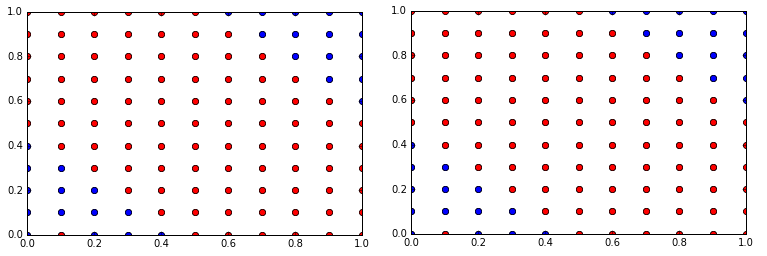
\includegraphics[width=0.8\textwidth]{results}
\end{figure}

\subsection{Exercise 3}
Investigate the use of back-propagation learning using a sigmoidal nonlinearity to achieve one-toone mappings, as described here:
\begin{enumerate}
\item $F(x) = 1/x 1<=x<=100$

\item $F(x) = log10(x) 1<=x<=10$

\item $F(x) = exp(-x) 1<=x<=10$

\item $F(x) = sin(x) 0<=x<=pi/2$
\end{enumerate}
For each mapping, do the following:
\begin{itemize}
\item Set up two sets of data, one for network training, and the other for testing.

\item Use the training data set to compute the synaptic weights of the network, assumed to have a single hidden layer.

\item Evaluate the computation accuracy of the network by using the test data. Use a single hidden layer but with a variable number of hidden neurons. Investigate how the network performance is affected by varying the size of the hidden layer.
\end{itemize}


You can use any neural network toolbox (MATLAB or python or ...) for solving this

problem or you can use your own implementation of MLP from previous question.
\subsection{Solution}

MLP backpropagation algorithm was implemented in MATLAB and has 2 functions:
\begin{itemize}
\item MLP evaluation;

\item MLP backpropagation.
\end{itemize}

The algorithm works for MLP with any number of hidden layers and sigmoid activation function.
\medskip

MLP evaluation:
\medskip

\lstinputlisting{fmlp.m}
\newpage

Training MLP by backpropagation.
\medskip
\lstinputlisting{trainMLP.m}

\medskip
In the exercise, SISO functions were modelled with a single hidden layer. Initial weights were taken as uniformly distributed numbers in $[0,1]$. Training and testing sets were created to verify MLP performance.
\medskip
Matlab script with experiment setup:

\lstinputlisting{Ex3.m}

\newpage
Results of the experiments:

\begin{enumerate}
\item $1/x$ function with 2 neurons in hidden layer. 

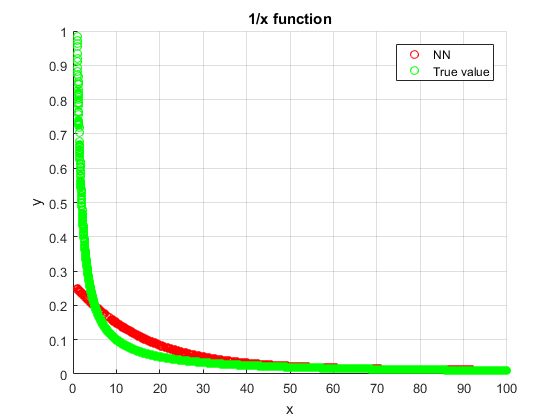
\includegraphics[scale = 0.8]{hyp2.png}

\item $1/x$ function with 5 neurons in hidden layer.

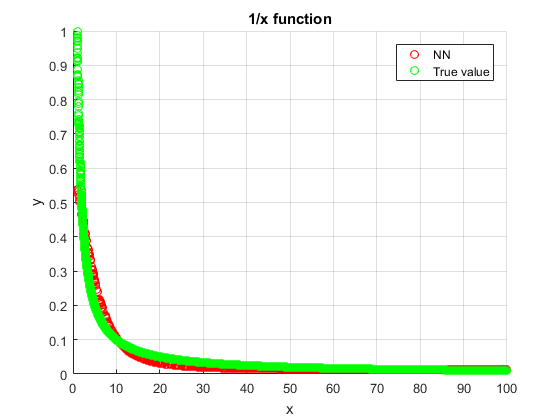
\includegraphics[scale = 0.8]{hyp5.png}

\item $log_{10}$ function with 2 neurons in hidden layer.

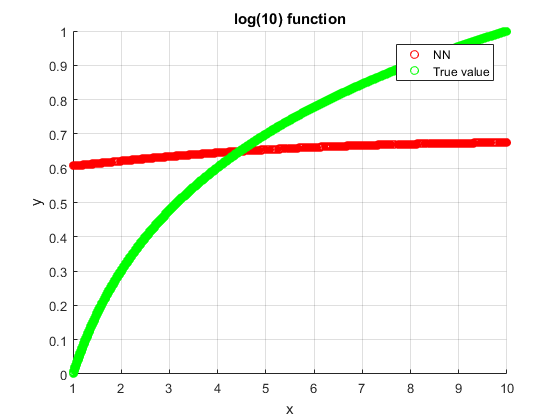
\includegraphics[scale = 0.8]{log2.png}

\item $log_{10}$ function with 5 neurons in hidden layer.

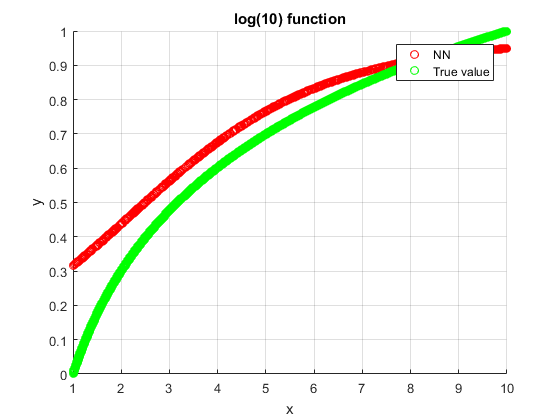
\includegraphics[scale = 0.8]{log5.png}

\item $\exp(-x)$ function with 2 neurons in hidden layer.

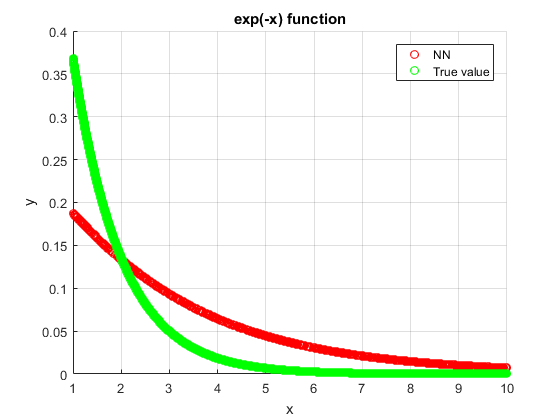
\includegraphics[scale = 0.8]{exp2.png}

\item $\exp(-x)$ function with 5 neurons in hidden layer.

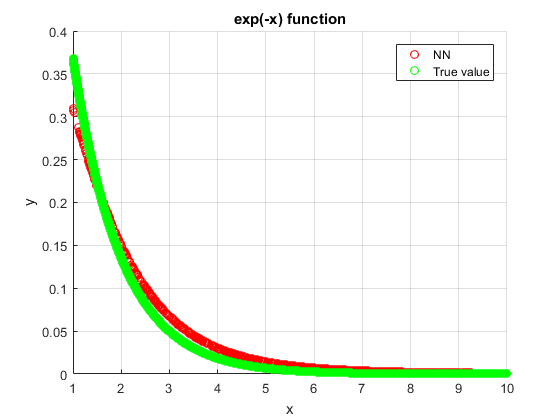
\includegraphics[scale = 0.8]{exp5.png}

\item $\sin(x)$ function with 2 neurons in hidden layer.

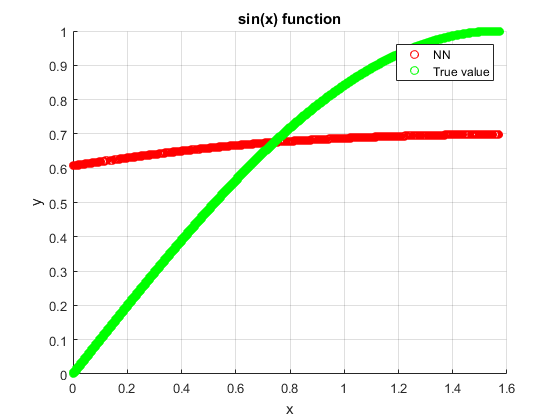
\includegraphics[scale = 0.8]{sin2.png}

\item $\sin(x)$ function with 5 neurons in hidden layer.

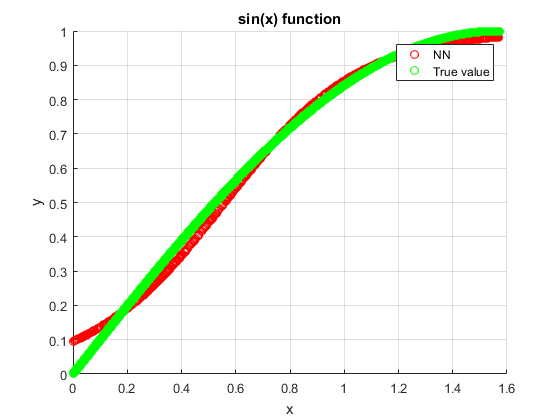
\includegraphics[scale = 0.8]{sin52.png}


\end{enumerate}

It can be seen, that extra hidden layers increase precision of the MLP. However, MLP is still sensitive to initial weights and parameter $\eta$.

\end{document}
